\newpage
\section{Supplemental images}
\label{sec:supp}
%
% \subsection{Bumpy surface}
% Motivation: Four images below are pixel-wise different. But from human perception, we consider the images in each row are equivalent.

% \begin{figure}[H]
% 	\addtolength{\tabcolsep}{-3.5pt}
% 	\begin{tabular}{ccc}
% 		
\includegraphics[width=0.30\columnwidth]{results/bump/syn_comp/bump04rd1.png} &
% 		
\includegraphics[width=0.30\columnwidth]{results/bump/syn_comp/bump04rd2.png} &
% 		\includegraphics[width=0.35\columnwidth]{results/bump/syn_comp/bump04diff.pdf} \\
% 		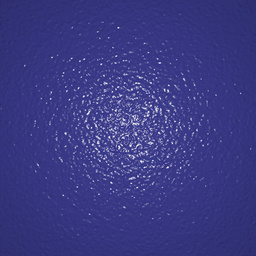
\includegraphics[width=0.30\columnwidth]{results/bump/syn_comp/bump02rd1.png} &
% 		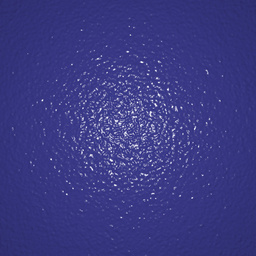
\includegraphics[width=0.30\columnwidth]{results/bump/syn_comp/bump02rd2.png} &
% 		\includegraphics[width=0.35\columnwidth]{results/bump/syn_comp/bump02diff.pdf} \\
% 	\end{tabular}
% 	\caption{\label{fig:syn1}
% 		Two images in each row have same parameters but with different randomness. The images in bottom row have smoother brdf.
% 	}
% \end{figure}


\newpage
\subsubsection{Synthetic data}
XXXXXXXXXX

\begin{figure}[H]
	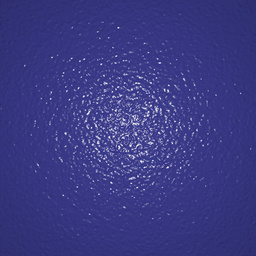
\includegraphics[width=0.4\columnwidth]{results/bump/syn_comp/bump02rd1.png}
	\caption{
		Target image (reference)
	}
\end{figure}


\begin{figure}[H]
	\addtolength{\tabcolsep}{-3.5pt}
	\begin{tabular}{ccc}
		\includegraphics[width=0.30\columnwidth]{results/bump/syn0/rd.png} &
		\includegraphics[width=0.30\columnwidth]{results/bump/syn0/rd1.png} &
		\includegraphics[width=0.30\columnwidth]{results/bump/syn0/rd2.png} \\
		\includegraphics[width=0.30\columnwidth]{results/bump/syn0/rd3.png} &
		\includegraphics[width=0.30\columnwidth]{results/bump/syn0/rd4.png} &
		\includegraphics[width=0.30\columnwidth]{results/bump/syn0/rd5.png} \\
		\includegraphics[width=0.30\columnwidth]{results/bump/syn0/rd6.png} &
		\includegraphics[width=0.30\columnwidth]{results/bump/syn0/rd7.png} &
		\includegraphics[width=0.30\columnwidth]{results/bump/syn0/rd8.png} \\
	\end{tabular}
	\caption{
		Random picked from HMC sampled results. Only use mean.
	}
\end{figure}

\begin{figure}[H]
	\addtolength{\tabcolsep}{-3.5pt}
	\begin{tabular}{ccc}
		\includegraphics[width=0.30\columnwidth]{results/bump/syn0/rd.pdf} &
		\includegraphics[width=0.30\columnwidth]{results/bump/syn0/rd1.pdf} &
		\includegraphics[width=0.30\columnwidth]{results/bump/syn0/rd2.pdf} \\
		\includegraphics[width=0.30\columnwidth]{results/bump/syn0/rd3.pdf} &
		\includegraphics[width=0.30\columnwidth]{results/bump/syn0/rd4.pdf} &
		\includegraphics[width=0.30\columnwidth]{results/bump/syn0/rd5.pdf} \\
		\includegraphics[width=0.30\columnwidth]{results/bump/syn0/rd6.pdf} &
		\includegraphics[width=0.30\columnwidth]{results/bump/syn0/rd7.pdf} &
		\includegraphics[width=0.30\columnwidth]{results/bump/syn0/rd8.pdf} \\
	\end{tabular}
	\caption{
		Corresponding posterior and picked point. Only use mean.
	}
\end{figure}



\begin{figure}[H]
	\addtolength{\tabcolsep}{-3.5pt}
	\begin{tabular}{ccc}
		\includegraphics[width=0.30\columnwidth]{results/bump/syn1/rd.png} &
		\includegraphics[width=0.30\columnwidth]{results/bump/syn1/rd1.png} &
		\includegraphics[width=0.30\columnwidth]{results/bump/syn1/rd2.png} \\
		\includegraphics[width=0.30\columnwidth]{results/bump/syn1/rd3.png} &
		\includegraphics[width=0.30\columnwidth]{results/bump/syn1/rd4.png} &
		\includegraphics[width=0.30\columnwidth]{results/bump/syn1/rd5.png} \\
		\includegraphics[width=0.30\columnwidth]{results/bump/syn1/rd6.png} &
		\includegraphics[width=0.30\columnwidth]{results/bump/syn1/rd7.png} &
		\includegraphics[width=0.30\columnwidth]{results/bump/syn1/rd8.png} \\
	\end{tabular}
	\caption{
		Random picked from HMC sampled results. Use mean and stddev.
	}
\end{figure}

\begin{figure}[H]
	\addtolength{\tabcolsep}{-3.5pt}
	\begin{tabular}{ccc}
		\includegraphics[width=0.30\columnwidth]{results/bump/syn1/rd.pdf} &
		\includegraphics[width=0.30\columnwidth]{results/bump/syn1/rd1.pdf} &
		\includegraphics[width=0.30\columnwidth]{results/bump/syn1/rd2.pdf} \\
		\includegraphics[width=0.30\columnwidth]{results/bump/syn1/rd3.pdf} &
		\includegraphics[width=0.30\columnwidth]{results/bump/syn1/rd4.pdf} &
		\includegraphics[width=0.30\columnwidth]{results/bump/syn1/rd5.pdf} \\
		\includegraphics[width=0.30\columnwidth]{results/bump/syn1/rd6.pdf} &
		\includegraphics[width=0.30\columnwidth]{results/bump/syn1/rd7.pdf} &
		\includegraphics[width=0.30\columnwidth]{results/bump/syn1/rd8.pdf} \\
	\end{tabular}
	\caption{
		Corresponding posterior and picked point. Use mean and stddev.
	}
\end{figure}

\begin{figure}[H]
	\includegraphics[width=0.7\columnwidth]{placeholder/placeholder.jpg}
	\caption{
		PLACEHOLDER
	}
\end{figure}


\begin{figure}[H]
	\addtolength{\tabcolsep}{-3.5pt}
	\begin{tabular}{ccc}
		\includegraphics[width=0.30\columnwidth]{results/bump/syn2/rd.png} &
		\includegraphics[width=0.30\columnwidth]{results/bump/syn2/rd1.png} &
		\includegraphics[width=0.30\columnwidth]{results/bump/syn2/rd2.png} \\
		\includegraphics[width=0.30\columnwidth]{results/bump/syn2/rd3.png} &
		\includegraphics[width=0.30\columnwidth]{results/bump/syn2/rd4.png} &
		\includegraphics[width=0.30\columnwidth]{results/bump/syn2/rd5.png} \\
		\includegraphics[width=0.30\columnwidth]{results/bump/syn2/rd6.png} &
		\includegraphics[width=0.30\columnwidth]{results/bump/syn2/rd7.png} &
		\includegraphics[width=0.30\columnwidth]{results/bump/syn2/rd8.png} \\
	\end{tabular}
	\caption{
		Random picked from HMC sampled results. Use mean and 2D FFT.
	}
\end{figure}

\begin{figure}[H]
	\addtolength{\tabcolsep}{-3.5pt}
	\begin{tabular}{ccc}
		\includegraphics[width=0.30\columnwidth]{results/bump/syn2/rd.pdf} &
		\includegraphics[width=0.30\columnwidth]{results/bump/syn2/rd1.pdf} &
		\includegraphics[width=0.30\columnwidth]{results/bump/syn2/rd2.pdf} \\
		\includegraphics[width=0.30\columnwidth]{results/bump/syn2/rd3.pdf} &
		\includegraphics[width=0.30\columnwidth]{results/bump/syn2/rd4.pdf} &
		\includegraphics[width=0.30\columnwidth]{results/bump/syn2/rd5.pdf} \\
		\includegraphics[width=0.30\columnwidth]{results/bump/syn2/rd6.pdf} &
		\includegraphics[width=0.30\columnwidth]{results/bump/syn2/rd7.pdf} &
		\includegraphics[width=0.30\columnwidth]{results/bump/syn2/rd8.pdf} \\
	\end{tabular}
	\caption{
		Corresponding posterior and picked point. Use mean and 2D FFT.
	}
\end{figure}

\begin{figure}[H]
	\includegraphics[width=0.7\columnwidth]{placeholder/placeholder.jpg}
	\caption{
		PLACEHOLDER
	}
\end{figure}

\subsubsection{Real photo}
XXXXXXXXXX

\begin{figure}[H]
	\includegraphics[width=0.45\columnwidth]{results/bump/real1/target.png}
	\caption{
		Target image (reference)
	}
\end{figure}


\begin{figure}[H]
	\addtolength{\tabcolsep}{-3.5pt}
	\begin{tabular}{ccc}
		\includegraphics[width=0.30\columnwidth]{results/bump/real1/rd.png} &
		\includegraphics[width=0.30\columnwidth]{results/bump/real1/rd1.png} &
		\includegraphics[width=0.30\columnwidth]{results/bump/real1/rd2.png} \\
		\includegraphics[width=0.30\columnwidth]{results/bump/real1/rd3.png} &
		\includegraphics[width=0.30\columnwidth]{results/bump/real1/rd4.png} &
		\includegraphics[width=0.30\columnwidth]{results/bump/real1/rd5.png} \\
		\includegraphics[width=0.30\columnwidth]{results/bump/real1/rd6.png} &
		\includegraphics[width=0.30\columnwidth]{results/bump/real1/rd7.png} &
		\includegraphics[width=0.30\columnwidth]{results/bump/real1/rd8.png} \\
	\end{tabular}
	\caption{
		Random picked from HMC sampled results. Use image mean and fft mean.
	}
\end{figure}

\begin{figure}[H]
	\addtolength{\tabcolsep}{-3.5pt}
	\begin{tabular}{ccc}
		\includegraphics[width=0.30\columnwidth]{results/bump/real1/rd.pdf} &
		\includegraphics[width=0.30\columnwidth]{results/bump/real1/rd1.pdf} &
		\includegraphics[width=0.30\columnwidth]{results/bump/real1/rd2.pdf} \\
		\includegraphics[width=0.30\columnwidth]{results/bump/real1/rd3.pdf} &
		\includegraphics[width=0.30\columnwidth]{results/bump/real1/rd4.pdf} &
		\includegraphics[width=0.30\columnwidth]{results/bump/real1/rd5.pdf} \\
		\includegraphics[width=0.30\columnwidth]{results/bump/real1/rd6.pdf} &
		\includegraphics[width=0.30\columnwidth]{results/bump/real1/rd7.pdf} &
		\includegraphics[width=0.30\columnwidth]{results/bump/real1/rd8.pdf} \\
	\end{tabular}
	\caption{
		Corresponding posterior and picked point. Use image mean and fft mean.
	}
\end{figure}



\subsection{Brushed metal}

\subsubsection{Real photo}
XXXXXXXXXX

\begin{figure}[H]
	\includegraphics[width=0.4\columnwidth]{results/brushed/real1/target.png}
	\caption{
		Target image (reference)
	}
\end{figure}


\begin{figure}[H]
	\addtolength{\tabcolsep}{-3.5pt}
	\begin{tabular}{ccc}
		\includegraphics[width=0.30\columnwidth]{results/brushed/real1/rd.png} &
		\includegraphics[width=0.30\columnwidth]{results/brushed/real1/rd1.png} &
		\includegraphics[width=0.30\columnwidth]{results/brushed/real1/rd2.png} \\
		\includegraphics[width=0.30\columnwidth]{results/brushed/real1/rd3.png} &
		\includegraphics[width=0.30\columnwidth]{results/brushed/real1/rd4.png} &
		\includegraphics[width=0.30\columnwidth]{results/brushed/real1/rd5.png} \\
		\includegraphics[width=0.30\columnwidth]{results/brushed/real1/rd6.png} &
		\includegraphics[width=0.30\columnwidth]{results/brushed/real1/rd7.png} &
		\includegraphics[width=0.30\columnwidth]{results/brushed/real1/rd8.png} \\
	\end{tabular}
	\caption{
		Random picked from HMC sampled results. Use image mean and fft mean.
	}
\end{figure}

\begin{figure}[H]
	\addtolength{\tabcolsep}{-3.5pt}
	\begin{tabular}{ccc}
		\includegraphics[width=0.30\columnwidth,height=0.15\columnwidth]{results/brushed/real1/rd.pdf} &
		\includegraphics[width=0.30\columnwidth,height=0.15\columnwidth]{results/brushed/real1/rd1.pdf} &
		\includegraphics[width=0.30\columnwidth,height=0.15\columnwidth]{results/brushed/real1/rd2.pdf} \\
		\includegraphics[width=0.30\columnwidth,height=0.15\columnwidth]{results/brushed/real1/rd3.pdf} &
		\includegraphics[width=0.30\columnwidth,height=0.15\columnwidth]{results/brushed/real1/rd4.pdf} &
		\includegraphics[width=0.30\columnwidth,height=0.15\columnwidth]{results/brushed/real1/rd5.pdf} \\
		\includegraphics[width=0.30\columnwidth,height=0.15\columnwidth]{results/brushed/real1/rd6.pdf} &
		\includegraphics[width=0.30\columnwidth,height=0.15\columnwidth]{results/brushed/real1/rd7.pdf} &
		\includegraphics[width=0.30\columnwidth,height=0.15\columnwidth]{results/brushed/real1/rd8.pdf} \\
	\end{tabular}
	\caption{
		Corresponding posterior and picked point. Use image mean and fft mean.
	}
\end{figure}

\subsection{Metallic flakes}

\subsubsection{Synthetic data}
XXXXXXXXXX

\begin{figure}[H]
	\includegraphics[width=0.45\columnwidth]{results/flake/syn1/target.png}
	\caption{
		Target image (reference)
	}
\end{figure}

\begin{figure}[H]
	\addtolength{\tabcolsep}{-3.5pt}
	\begin{tabular}{ccc}
		\includegraphics[width=0.30\columnwidth]{results/flake/syn1/rd0.png} &
		\includegraphics[width=0.30\columnwidth]{results/flake/syn1/rd1.png} &
		\includegraphics[width=0.30\columnwidth]{results/flake/syn1/rd2.png} \\
		\includegraphics[width=0.30\columnwidth]{results/flake/syn1/rd3.png} &
		\includegraphics[width=0.30\columnwidth]{results/flake/syn1/rd4.png} &
		\includegraphics[width=0.30\columnwidth]{results/flake/syn1/rd5.png} \\
		\includegraphics[width=0.30\columnwidth]{results/flake/syn1/rd6.png} &
		\includegraphics[width=0.30\columnwidth]{results/flake/syn1/rd7.png} &
		\includegraphics[width=0.30\columnwidth]{results/flake/syn1/rd8.png} \\
	\end{tabular}
	\caption{
		Random picked from HMC sampled results.
	}
\end{figure}

\begin{figure}[H]
	\addtolength{\tabcolsep}{-3.5pt}
	\begin{tabular}{ccc}
		\includegraphics[width=0.30\columnwidth]{results/flake/syn1/rd0.pdf} &
		\includegraphics[width=0.30\columnwidth]{results/flake/syn1/rd1.pdf} &
		\includegraphics[width=0.30\columnwidth]{results/flake/syn1/rd2.pdf} \\
		\includegraphics[width=0.30\columnwidth]{results/flake/syn1/rd3.pdf} &
		\includegraphics[width=0.30\columnwidth]{results/flake/syn1/rd4.pdf} &
		\includegraphics[width=0.30\columnwidth]{results/flake/syn1/rd5.pdf} \\
		\includegraphics[width=0.30\columnwidth]{results/flake/syn1/rd6.pdf} &
		\includegraphics[width=0.30\columnwidth]{results/flake/syn1/rd7.pdf} &
		\includegraphics[width=0.30\columnwidth]{results/flake/syn1/rd8.pdf} \\
	\end{tabular}
	\caption{
		Corresponding posterior and picked point.
	}
\end{figure}

\subsubsection{Real photo}
XXXXXXXXXX

\begin{figure}[H]
	\includegraphics[width=0.45\columnwidth]{results/flake/real1/target.png}
	\caption{
		Target image (reference)
	}
\end{figure}

\begin{figure}[H]
	\addtolength{\tabcolsep}{-3.5pt}
	\begin{tabular}{ccc}
		\includegraphics[width=0.30\columnwidth]{results/flake/real1/rd.png} &
		\includegraphics[width=0.30\columnwidth]{results/flake/real1/rd1.png} &
		\includegraphics[width=0.30\columnwidth]{results/flake/real1/rd2.png} \\
		\includegraphics[width=0.30\columnwidth]{results/flake/real1/rd3.png} &
		\includegraphics[width=0.30\columnwidth]{results/flake/real1/rd4.png} &
		\includegraphics[width=0.30\columnwidth]{results/flake/real1/rd5.png} \\
		\includegraphics[width=0.30\columnwidth]{results/flake/real1/rd6.png} &
		\includegraphics[width=0.30\columnwidth]{results/flake/real1/rd7.png} &
		\includegraphics[width=0.30\columnwidth]{results/flake/real1/rd8.png} \\
	\end{tabular}
	\caption{
		Random picked from HMC sampled results.
	}
\end{figure}

\begin{figure}[H]
	\addtolength{\tabcolsep}{-3.5pt}
	\begin{tabular}{ccc}
		\includegraphics[width=0.30\columnwidth]{results/flake/real1/rd.pdf} &
		\includegraphics[width=0.30\columnwidth]{results/flake/real1/rd1.pdf} &
		\includegraphics[width=0.30\columnwidth]{results/flake/real1/rd2.pdf} \\
		\includegraphics[width=0.30\columnwidth]{results/flake/real1/rd3.pdf} &
		\includegraphics[width=0.30\columnwidth]{results/flake/real1/rd4.pdf} &
		\includegraphics[width=0.30\columnwidth]{results/flake/real1/rd5.pdf} \\
		\includegraphics[width=0.30\columnwidth]{results/flake/real1/rd6.pdf} &
		\includegraphics[width=0.30\columnwidth]{results/flake/real1/rd7.pdf} &
		\includegraphics[width=0.30\columnwidth]{results/flake/real1/rd8.pdf} \\
	\end{tabular}
	\caption{
		Corresponding posterior and picked point.
	}
\end{figure}

\subsection{Scattering medium}

\begin{figure}[H]
	\includegraphics[width=0.95\columnwidth]{results/scatter/synthetic1/image.png}
	\caption{
		In this example, first we want to show that the similarity theory curve is properly covered by our sampled posterior. Secondly, if two points on the similarity curve are not close to each other, the rendered results have 20 percent mismatch around the peak. But in our method, we can easily find a better match.
	}
\end{figure}
%In Figures~\ref{fig:a}

